\usepackage[utf8x]{inputenc}
\usepackage{ucs}
\usepackage{amsmath}
\usepackage{amsfonts}
\usepackage{amssymb}
\usepackage{multicol}
\usepackage{graphicx}
%\usepackage{hyperref}		% automatic included by beamer
\usepackage{tikz}
\usetikzlibrary{arrows,positioning,shapes,graphs}
\usepackage{listings}
\usepackage{multicol}
\usepackage[absolute,overlay]{textpos}
\usepackage{appendixnumberbeamer}
\usepackage{url}

\setlength{\TPHorizModule}{1cm}
\setlength{\TPVertModule}{1cm}

\title{Embedded GNU/Linux Basics}
%\subtitle{}
\author{Urs Fässler}
\date{21.11.2015}
\institute
{
  17. LinuxDay\\
  Dornbirn
}
%\subject{}

\newcommand{\hnote}[1]{\only<handout>{\footnote{#1}}}
\newcommand{\hcite}[1]{\only<handout>{\cite{#1}}}
\bibliographystyle{plainurl}  % urlbst
\setbeamertemplate{bibliography item}{[\theenumiv]}

\lstset
{  
	basicstyle=\scriptsize\ttfamily,
	keywordstyle={\bf\color{green!50!black}},
	identifierstyle=\color{blue!25!black},
	stringstyle=\color{orange!75!black},
%  language=,
%  morekeywords={signals,slots,interface,event,message,String,Integer,component,import,uses,provides,implementation,connection,elementary,begin,end,func,pure,const},
%  numbers=none,
  numberstyle={\color{Grey}},
%  keywordstyle={\color{DarkRed}\bfseries},
%  identifierstyle={\color{Blue}}
%  columns=flexible,
	float=tb,
	frame=none,
	numbers=left,                           % Line nums position
	numberstyle=\tiny,                      % Line-numbers fonts
	stepnumber=1                           % Step between two line-numbers
}


\newcommand*\oldmacro{}%
\let\oldmacro\insertshorttitle%
\renewcommand*\insertshorttitle{%
	\oldmacro\hfill%
	\insertframenumber
}
\usetheme{Luebeck}

% remove navigation bars
\beamertemplatenavigationsymbolsempty

% remove section information
\setbeamertemplate{headline}{\insertsection}
\setbeamertemplate{frametitle}
{\vskip-3pt
  \leavevmode
  \hbox{%
  \begin{beamercolorbox}[wd=\paperwidth,ht=3ex,dp=1ex]{frametitle}%
    \raggedright
    \hspace*{0.5em}
    \Large\insertframetitle\hfill\normalsize\insertsection
    \hspace*{0.5em}
  \end{beamercolorbox}
  }%
}

%\AtBeginSection{\frame{\sectionpage}}

\lstdefinelanguage{bitbake}{
	morekeywords={
		LICENSE, inherit, IMAGE_INSTALL, IMAGE_FEATURES, SUMMARY
	},
	otherkeywords={},
	sensitive=true,
	morecomment=[l]{\#},
	morestring=[b]",
	escapeinside={@}{@}, 
	showspaces=false,                       % Dont make spaces visible
	showstringspaces=false,
	showtabs=false,                         % Dont make tabls visible
	breaklines=true,                        % Automatic line breaking?
}



\begin{document}

\frame{\titlepage}

%\section{Einführung}
\section*{Intro}
\begin{frame}{Eigenschaften Embedded System\hcite{embeddedSpecials}}
	\pause
	\begin{multicols}{2}
		\begin{itemize}
			\item Kosten
			\item Grösse
			\item Energie
			\item Zuverlässigkeit
			\item Sicherheit
			\item Langlebigkeit
			\item Echtzeit
		\end{itemize}
	\end{multicols}
\end{frame}

\begin{frame}{Definition Embedded System}
	Der Ausdruck embedded system bezeichnet einen Computer, der in einem technischen Kontext eingebettet ist. \hcite{wikiEmbedded}
	\begin{flushright}
		Nach Wikipedia
	\end{flushright}
\end{frame}

\begin{frame}{Embedded Systeme}
	\footnotesize{
	\begin{multicols}{2}
				\only<handout>{Digitales Multimeter}
				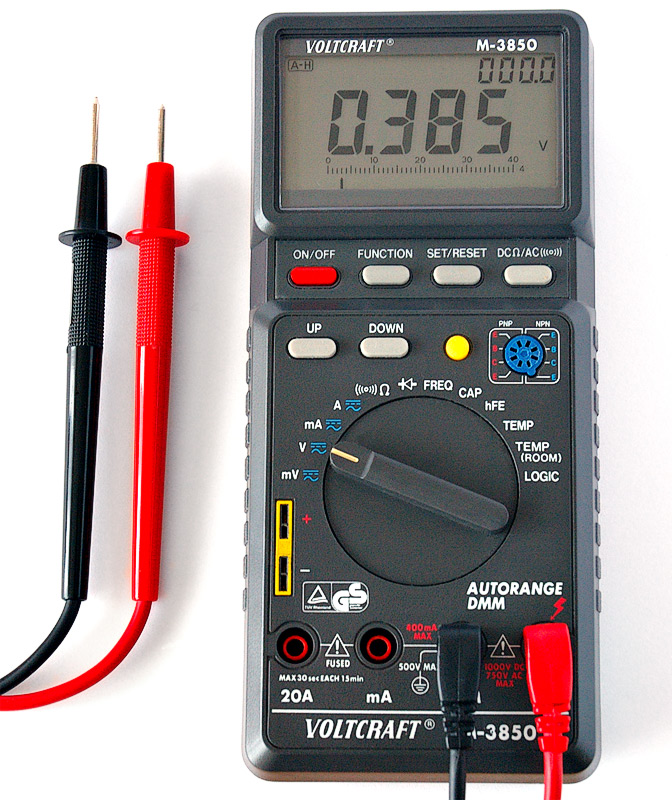
\includegraphics[height=4cm]{res/Digital_Multimeter_Aka.jpg}\hcite{multimeter}
				\only<handout>{
					\begin{itemize}
						\item Sensor produziert ~20 B/sec
						\item Reduzierung auf ~2 B/sec
						\item Verarbeitung auf internem uC
					\end{itemize}
				}
				\pagebreak
				\only<handout>{ATLAS/LHC/CERN}
				\visible<2->{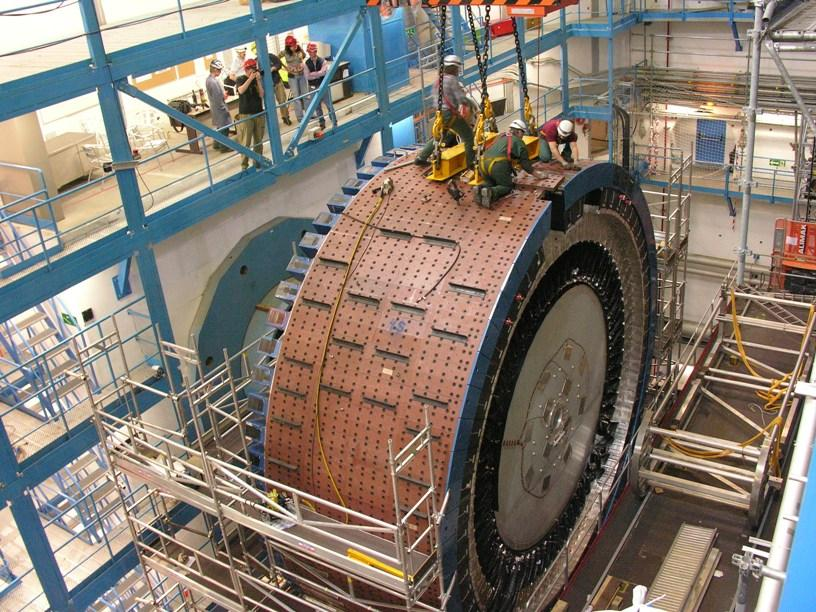
\includegraphics[height=4cm]{res/ATLAS_Tile_Calorimeter}\hcite{tileCalorimeter}}
				\only<handout>{
					\begin{itemize}
						\item Sensor produziert 1 PiB/sec
						\item Reduzierung auf ~100 MiB/sec \hcite{wikiAtlas}
						\item Verarbeitung auf eigenen 20'000 Server und Grid \hcite{wikiCernServer}
					\end{itemize}
				}
	\end{multicols}
	}
\end{frame}

\begin{frame}{Typisches GNU/Linux Embedded System}
	\begin{center}
		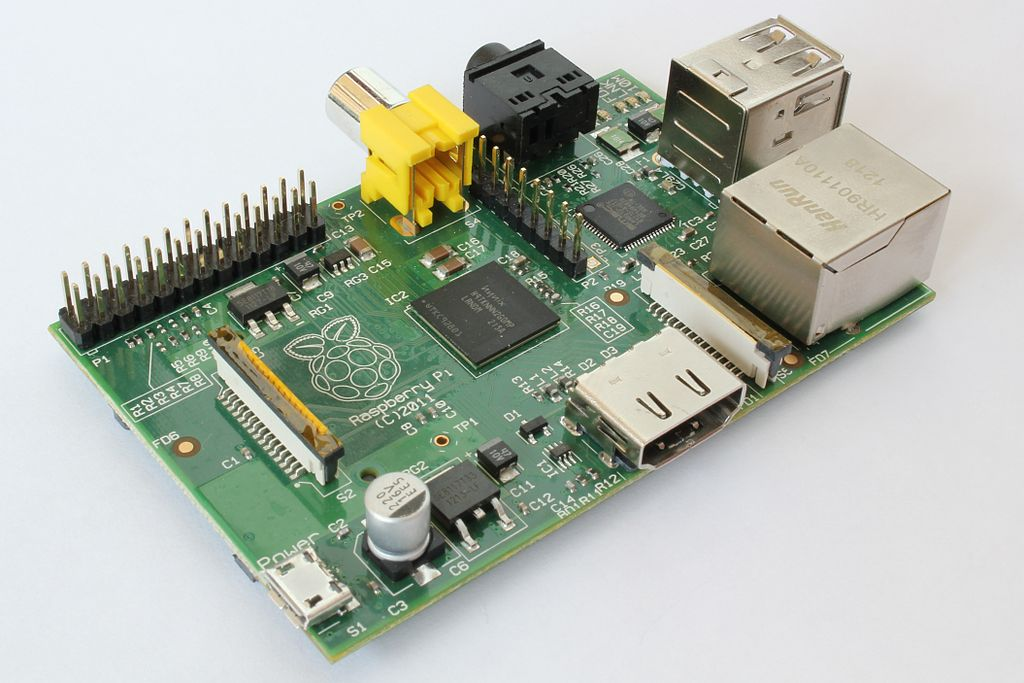
\includegraphics[width=5cm]{res/RaspberryPi.jpg}\hcite{raspberryPi}
		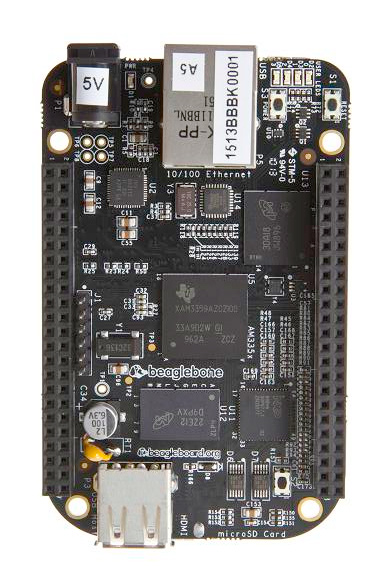
\includegraphics[width=3.5cm]{res/Beaglebone_Black.jpg}\hcite{beagleboneBlack}
	\end{center}
\end{frame}

\begin{frame}{Echtzeit}
	\begin{center}
		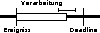
\includegraphics[width=8cm]{res/echtzeit.pdf}
	\end{center}
	\only<handout>{
		\begin{itemize}
			\item Bearbeitung ist nach einer bestimmten Zeit nach dem auftreten eines Ereignisses abgeschlossen.
			\item bei weicher Echtzeit ist dieses Verhalten wünschenswert (Video Wiedergabe)
			\item Echtzeit ist oft nicht nötig
			\item Linux ist nicht Echtzeit-Fähig
			\item Lösung ist separater uC, im SOC oder dediziertem Chip
		\end{itemize}
	}
\end{frame}

\begin{frame}{Aufgabe}
	\visible<2->{
		\begin{itemize}
			\item Webserver für Most Useless Machine Ever!
		\end{itemize}
	}
	\begin{center}
		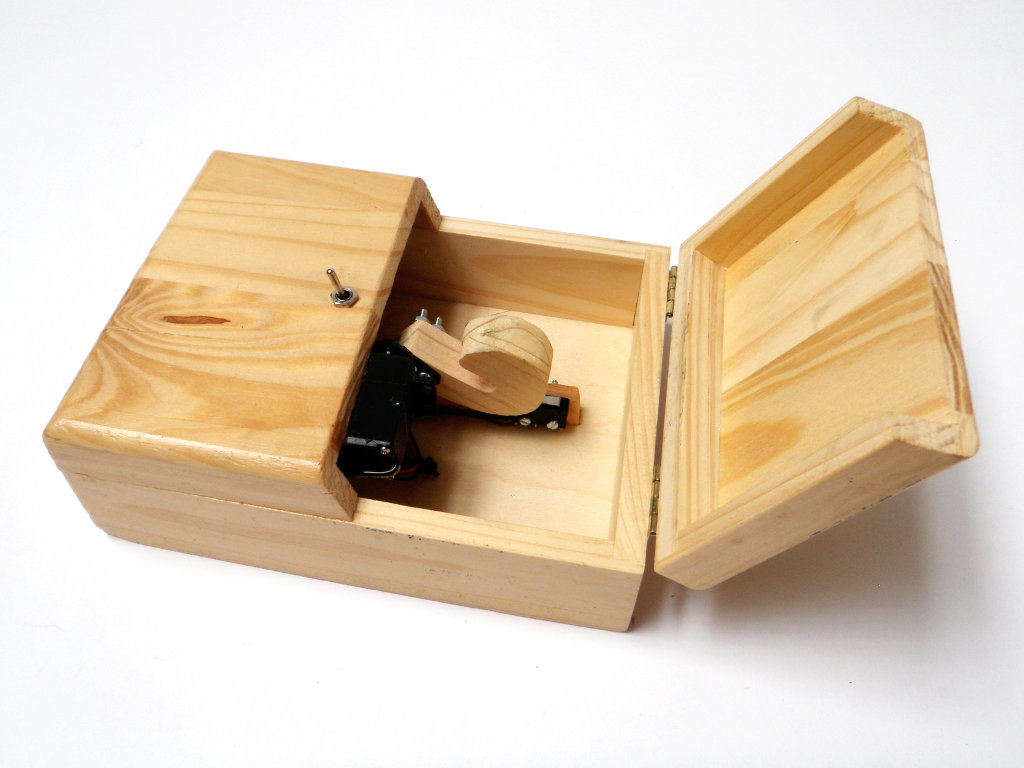
\includegraphics[height=4cm]{res/mume.jpg}
		\hcite{mumePic}
		\visible<2->{
			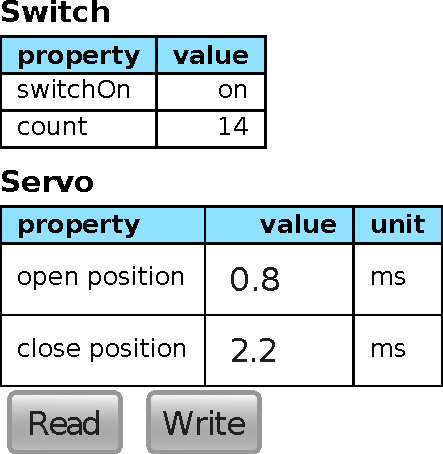
\includegraphics[height=4cm]{res/mumehtml.pdf}
		}
	\end{center}
\end{frame}

\begin{frame}{Vorgehen}
\tableofcontents
\end{frame}

\section{Hardware}

\begin{frame}{System}
	\begin{center}
		\begin{tabular}{cc}
			Bare Metal uC & GNU/Linux SOC \\
			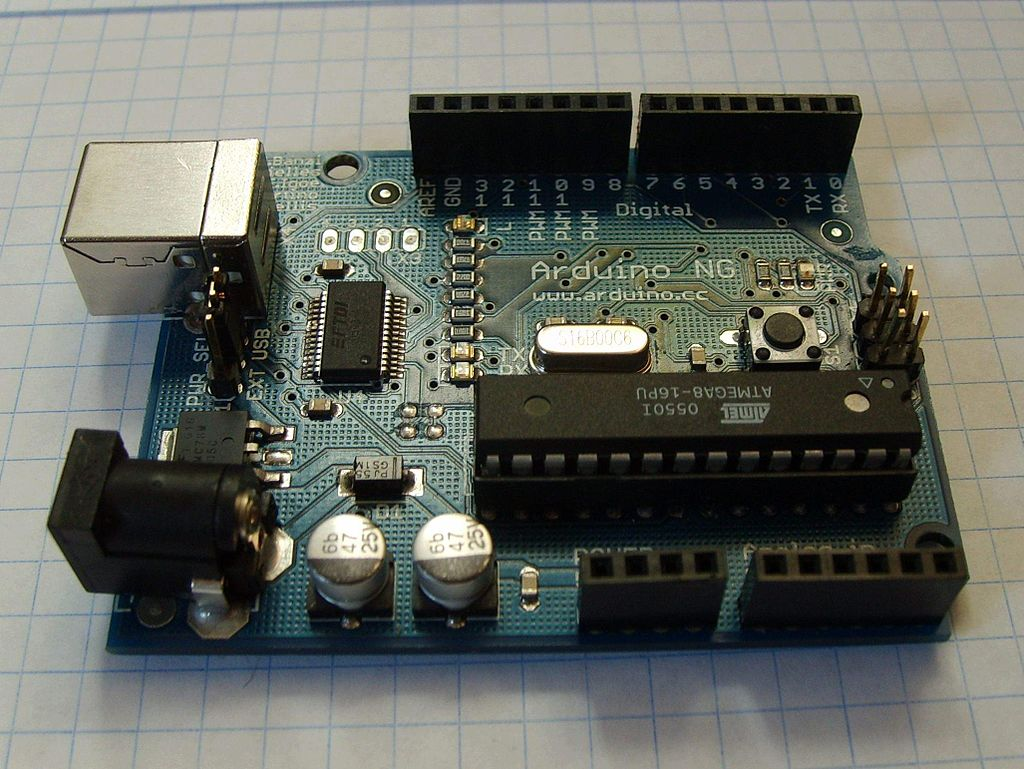
\includegraphics[height=3cm]{res/arduino.jpg} & 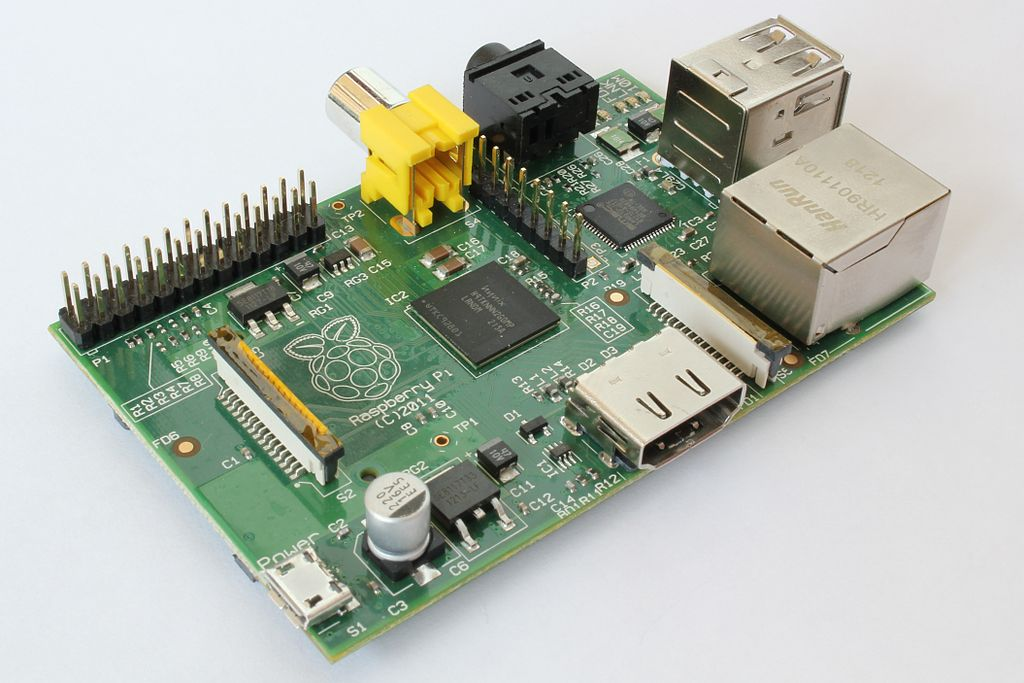
\includegraphics[height=3cm]{res/RaspberryPi.jpg}\hcite{raspberryPi} \\
			\only<handout>{
				Echtzeit & Memory und Prozess Management\\
				niedrige System-Komplexität & Treiber \& Protokolle\\
				keine Infrastruktur & hohe System-Komplexität
			}
		\end{tabular} 
	\end{center}
\end{frame}

\begin{frame}{Board}
	\begin{center}
		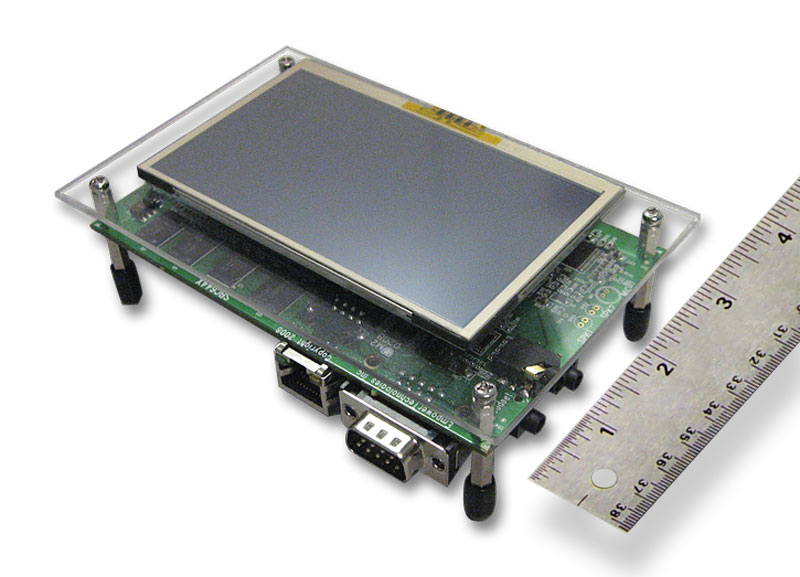
\includegraphics[height=2.7cm]{res/Development_Kit_EDK6446.jpg}\hcite{industrialBoard}
		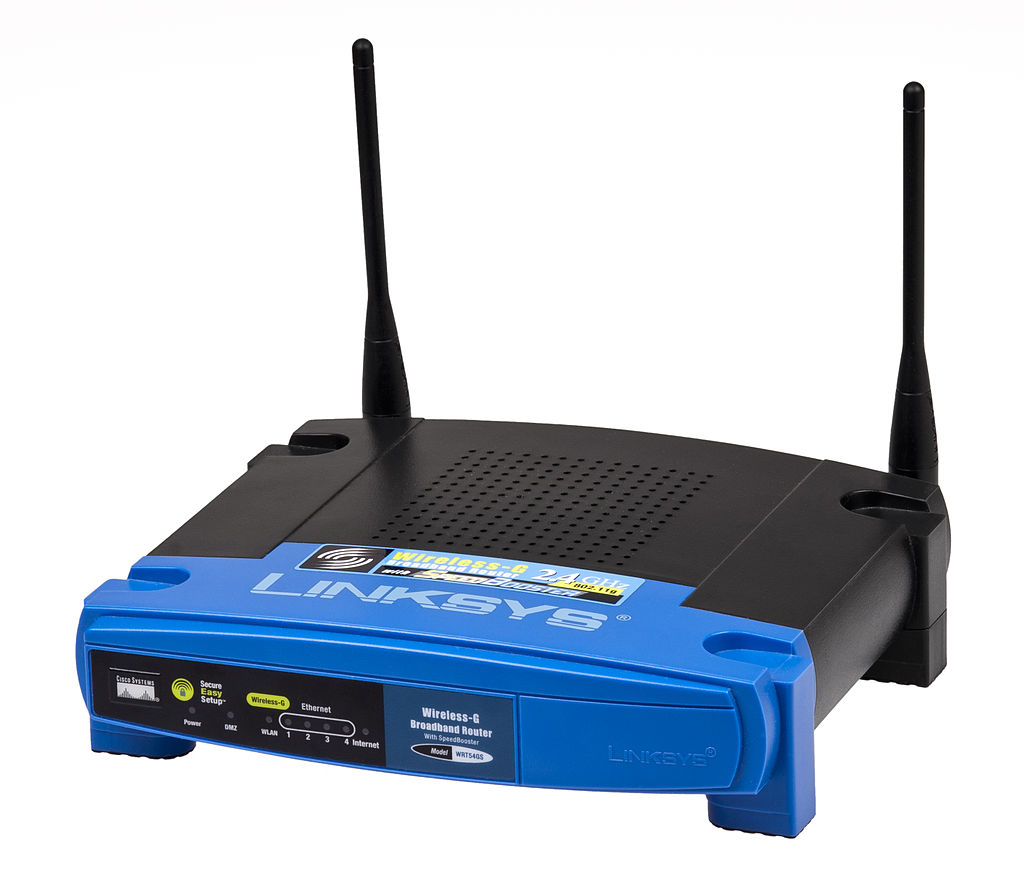
\includegraphics[height=2.8cm]{res/router.jpg}\hcite{router}
		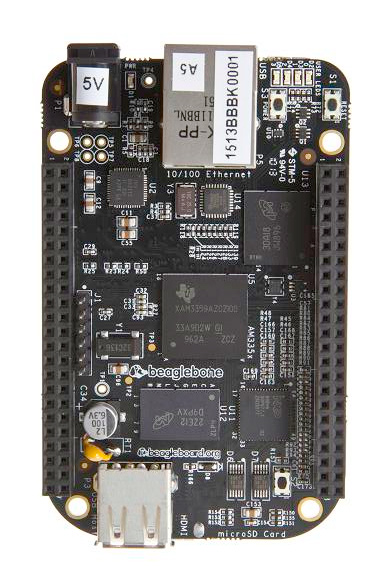
\includegraphics[height=3cm]{res/Beaglebone_Black.jpg}\hcite{beagleboneBlack}
	\end{center}
	\only<handout>{
		\begin{itemize}
			\item Industrie-Boards
			\item Consumer Hardware (Router, Media-Center, \ldots)
			\item Eval-/Bastelboards (Raspi, BeagleBone)
			\item[$\rightarrow$] BeagleBone Green
			\begin{itemize}
				\item Netzwerk
				\item Yocto Supported
				\item viele Anshlüsse
				\item USB Powered
			\end{itemize}
		\end{itemize}
	}
\end{frame}

\section{OS}

\begin{frame}{GNU/Linux Distribution}
	\begin{itemize}
		\item off-the-shelf (Debian, OpenWRT, \ldots)
		\visible<2->{
			\begin{itemize}
				\item weite Verbreitung; bekannt
				\item Updates werden von anderen bereitgestellt
				\item erlaubt Lizenz Verteilung?
			\end{itemize}
		}
		\item Yocto\hcite{whyYocto}\only<handout>{\footnote{Tools und Rezepte um eigene GNU/Linux Distribution zu bauen}}
		\visible<3->{
			\begin{itemize}
				\item git repository mit Konfiguration des gesamten System
				\item Patchen einzelner Pakete
				\item Optimierungen auf spezifische Hardware
				\item volle Kontrolle
			\end{itemize}
		}
	\end{itemize}
\end{frame}


\begin{frame}[fragile]{Yocto Image}
	\begin{multicols}{2}
		\begin{lstlisting}[title=mume-dev-image.bb,frame=single,language=bitbake]
LICENSE = "MIT"

inherit core-image
inherit populate_sdk_qt5

IMAGE_INSTALL = " \
  packagegroup-core-boot \
  @\ldots@-core-ssh-openssh \
  packagegroup-mume-common \
  packagegroup-dev-mume \
"

IMAGE_FEATURES += " \
  package-management \
  debug-tweaks \
"
		\end{lstlisting}
		\pause
		\begin{lstlisting}[title=packagegroup-dev-mume.bb, frame=single, numbers=right, language=bitbake]
SUMMARY = "developer tools for MUME"
LICENSE = "MIT"

inherit packagegroup

RDEPENDS_${PN} = "\
  bash \
  devmem2 \
  htop \
  nginx \
  openssh-sftp \
  perf \
  qtbase \
  time \
  @\ldots@
		\end{lstlisting}
	\end{multicols}
\end{frame}

\begin{frame}[fragile]{Yocto Image bauen}
	\begin{lstlisting}[frame=single,language=bash, basicstyle=\small\ttfamily]
$ bitbake mume-dev-image
	\end{lstlisting}
	\pause
	\begin{table}
		\caption{tmp/deploy/images/beaglebone/}
		\begin{tabular}{ll}
			\hline MLO & stage 1 loader \\ 
			\hline u-boot.img & stage 2 loader \\ 
			\hline uEnv.txt & u-boot Konfiguration \\ 
			\hline zImage & Kernel \\ 
			\hline zImage-bonegreen-mume.dtb & Device Tree \\ 
			\hline mume-dev-image-beaglebone.tar.bz2 & rootfs \\ 
			\hline 
		\end{tabular} 
	\end{table}
\end{frame}

\begin{frame}[fragile]{rootfs}
	\begin{lstlisting}[frame=,numbers=none,escapeinside={@}{@},language=,basicstyle=\small\ttfamily]
/
  bin
  boot
  etc
  home
  lib
  mnt
  opt
  root
  tmp
  usr
  var
  @\ldots@
	\end{lstlisting}
	\only<handout>{
		\begin{itemize}
			\item userspace
			\item ev. Kernel \& Device Tree
			\item nicht bootloader
		\end{itemize}
	}
\end{frame}

\begin{frame}[fragile]{Device Tree}
	\begin{lstlisting}[frame=,numbers=none,escapeinside={|}{|},language=,basicstyle=\small\ttfamily]
/ {
  compatible = "ti,am33xx";

  spi0: spi@48030000 {
    compatible = "ti,omap4-mcspi"|\hnote{Mapping zu Treiber}|;
    status = "disabled"|\hnote{aktivieren durch status="okay"}|;
    reg = <0x48030000 0x400>|\hnote{Register-Position, siehe Datenblatt des SOC}|;
    interrupts = <65>;
    dmas = <&edma|\hnote{Referenz zum DMA Device-Tree Knoten}| 16 &edma 17>;
    |\dots|
  };
|\dots|
	\end{lstlisting}
\end{frame}
\note{
	\begin{itemize}
		\item Linux kennt Hardware nicht
		\item Device Tree beschreibt Hardware
		\item Linux lädt Treiber anhand Device Tree
	\end{itemize}
}

\begin{frame}{Boot Process\hcite{OMAPBootloaderOverview}}
	\begin{center}
		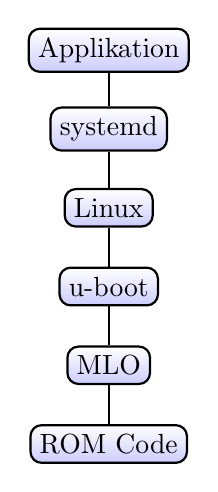
\begin{tikzpicture}[thick]
			\tikzstyle{every node}=[shape=rectangle, rounded corners,
				draw, align=center, top color=white, bottom color=blue!20]

			\visible<2->{
				\node at (0,0) (rom) {ROM Code};
			}

			\visible<3->{
				\node at (0,1) (mlo) {MLO};
				\draw (rom) -- (mlo);
			}

			\visible<4->{
				\node at (0,2) (uboot) {u-boot};
				\draw (mlo) -- (uboot);
			}

			\visible<5->{
				\node at (0,3) (linux) {Linux};
				\draw (uboot) -- (linux);
			}

			\visible<6->{
				\node at (0,4) (systemd) {systemd};
				\draw (linux) -- (systemd);
			}

			\visible<7->{
				\node at (0,5) (app) {Applikation};
				\draw (systemd) -- (app);
			}
		\end{tikzpicture}
	\end{center}\end{frame}
\note{
	\scriptsize{
		\begin{tabular}{|l|l|l|}
			\hline Typ & Name & Funktion \\ 
			\hline System startup & ROM Code & minimale Hardware Initialisierung \\ 
			& & in Boot-Devices nach Stage 1 Loader suchen \\
			& & Stage 1 Loader ins RAM laden und ausführen \\
			
			\hline Stage 1 Loader & MLO & Pin Muxing \\ 
			& x-loader & Clock und Memory initialisieren \\
			& (u-boot) & Stage 2 Loader ins RAM laden und ausführen \\
			
			\hline Stage 2 Loader & u-boot.img & Plattform Initialisierung (USB, Netzwerk, \ldots) \\
			& & Boot-Menü / Kommandozeile anzeigen \\
			& & Kernel und Device-Tree ins RAM laden und ausführen \\
			
			\hline Kernel & zImage & Treiber für Hardware laden \\ 
			& Linux & rootfs mounten \\
			& & Init-Process starten \\
			
			\hline Init & Systemd & Abhängigkeiten zwischen Services auflösen \\ 
			& & Services starten \\
			& & Services überwachen \\
			
			\hline 
		\end{tabular} 
	}
}

\begin{frame}[fragile]{SDK bauen}
	\pause
	\begin{lstlisting}[frame=single,language=bash, breaklines=true, basicstyle=\small\ttfamily]
$ bitbake mume-dev-image -c populate_sdk
$ ls -sh tmp/deploy/sdk/
695M mume-glibc-x86_64-mume-dev-image-cortexa8hf-vfp-neon-toolchain-2.0.sh
	\end{lstlisting}
	\pause
	\begin{itemize}
		\item Cross-Compiler
		\item rootfs (Libraries, \ldots)
		\item Entwicklerpakete (Header, \ldots)
		\item Paketmanager
	\end{itemize}
\end{frame}

\begin{frame}{Services (Applikation)}
	\begin{itemize}
		\item Embedded System besteht meist aus mehreren Prozessen $\rightarrow$ Microservices
		\item Webserver, Prozessueberwachung, SSH, FTP, UI
		\item standard linux tools (busybox)
		\item libraries
		\item packetmanager
		\item Hardware Ansteuerung
		\item gutes IPC system (z.B. kdbus)
		\item eigener Service
		\begin{itemize}
			\item reaktiv, event-getriggert
			\item Qt gut geeignet
		\end{itemize}
	\end{itemize}
\end{frame}

\begin{frame}{Hardware ansteuern}
	\begin{multicols}{2}
		\begin{center}
			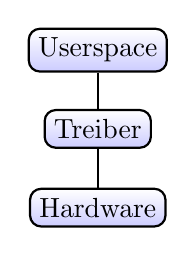
\begin{tikzpicture}[thick,
				every node/.style = {shape=rectangle, rounded corners,
					draw, align=center,
					top color=white, bottom color=blue!20}]]

				\node (userspace) {Userspace};
				\node[below of=userspace] (driver) {Treiber};
				\node[below of=driver] (hardware) {Hardware};
				
				\draw (userspace) to (driver);
				\draw (driver) to (hardware);
			\end{tikzpicture}
			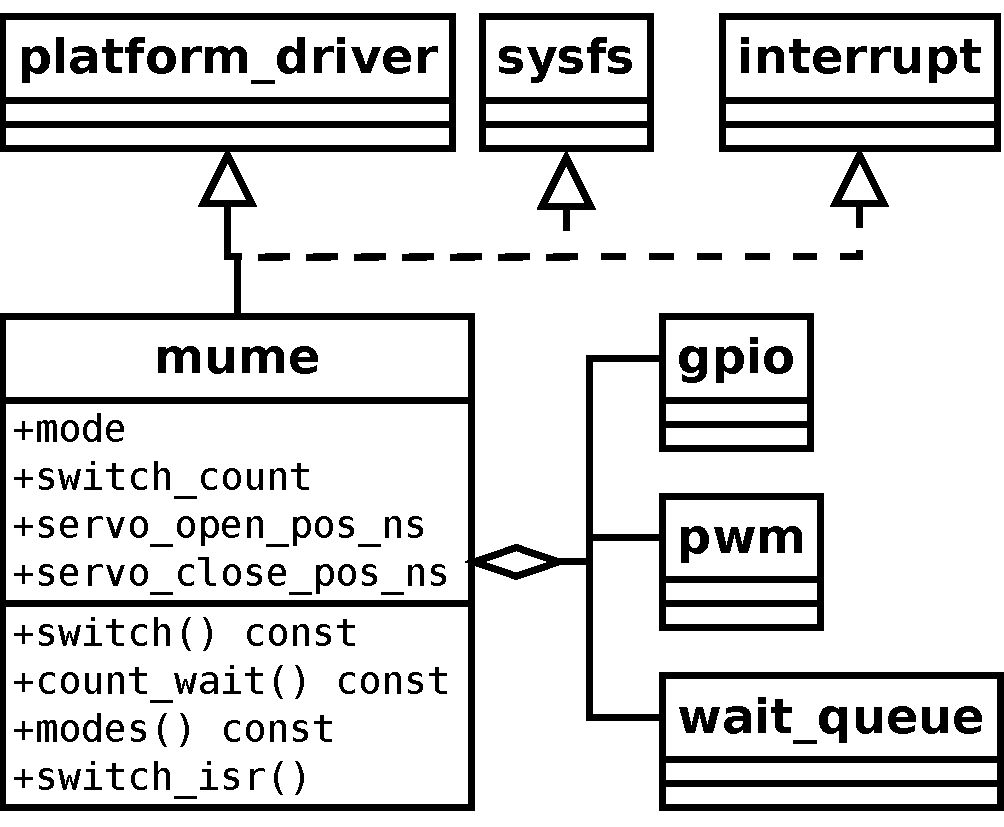
\includegraphics[width=0.5\textwidth]{res/mumedriver}
		\end{center}
	\end{multicols}
	\begin{itemize}
		\item wie können wir die Hardware ansteuern?
		\item[$\rightarrow$] Linux Treiber, Frameworks, Infrastructure:
		\begin{itemize}
			\item Framework für Treiber
			\item Infrastrukur um auf Subsysteme zuzugreifen
		\end{itemize}
	\end{itemize}
\end{frame}

\begin{frame}{MUME Service}
	\begin{itemize}
		\item wie können wir den Treiber ansprechen?
		\item[$\rightarrow$] sysfs
		\item mumesrv als Userspace-Teil des Treibers:
		\begin{itemize}
			\item Zugriff via D-Bus
			\item ablegen persistenter Daten (counter, open/close position)
			\item Kommunikation mit Treiber
		\end{itemize}
	\end{itemize}
\end{frame}

\begin{frame}{GUI}
	\begin{itemize}
		\item Browser Zugriff auf System?
		\item[$\rightarrow$] Web-Service
		\begin{itemize}
			\item nginx
			\item fastcgi
			\item mumeweb
			\begin{itemize}
				\item Kommunikation via D-Bus mit mumesrv
			\end{itemize}
		\end{itemize}
	\end{itemize}
\end{frame}

\begin{frame}{Service Manager}
	\begin{itemize}
		\item Wie starten und managen wir die Services?
		\item[$\rightarrow$] systemd
		\begin{itemize}
			\item service files schreiben
		\end{itemize}
	\end{itemize}
\end{frame}

\begin{frame}{Produktiv Image}
	\begin{itemize}
		\item Wie können wir die Firmware verteilen?
		\item[$\rightarrow$] Yocto
		\begin{itemize}
			\item Rezepte für Services
			\item anpassen bestehender Rezepte (nginx, qt, \ldots)
			\item Rezept für image
		\end{itemize}
		\item bitbake image
	\end{itemize}
\end{frame}

\begin{frame}{Was passiert bei einem Tastendruck in der Web-Applikation}
	Geht runter:
	\begin{itemize}
		\item SVG, Javascript
		\item XML/HTTP
		\item FastCGI
		\item MumeWeb
		\item D-Bus
		\item MumeSrv
		\item SysFS
		\item Kernel
		\item MUME-Treiber
		\item PWM
		\item Servo bewegt sich!
	\end{itemize}
\end{frame}

\begin{frame}{Echtzeit}
	\begin{itemize}
		\item Bearbeitung ist nach einer bestimmten Zeit nach dem auftreten eines Ereignisses abgeschlossen.
		\item Die Bearbeitung eines Interrupts dauert nie laenger als $t$.
		\item bei weicher Echtzeit ist dieses Verhalten wuenschenswert (Video wiedergabe)
		\item jeder Treiber kann Interrupts sperren
		\item Swapping
		\item Prozessoren mit Caches haben undefinierbares Verhalten, abschalten nicht Sinn der Sache
		\item Loesung ist separater uC, im selben oder eigenen DIE
	\end{itemize}
\end{frame}

\section*{Outro}
\begin{frame}
Link zu Projekt

Fragen?
\end{frame}


\only<handout>
{
\appendix

\section{Backup}



\begin{frame}{Boot Process \cite{OMAPBootloaderOverview}}
	\begin{tabular}{|l|l|l|}
		\hline typ & name & funktion \\ 
		\hline system startup & ROM Code & minimal hardware initialisierung \\ 
		& & in boot devices nach image suchen \\
		& & stage 1 loader ins ram laden und ausführen \\
		
		\hline stage 1 loader & x-loader (u-boot) & pin muxing \\ 
		& & clock und memory initialisieren \\
		& & stage 2 loader ins ram laden und ausführen \\
		
		\hline stage 2 loader & u-boot & platform initialisierung (USB, Netzwerk, \ldots) \\
		& & boot menu / Kommandozeile anzeigen \\
		& & Kernel und Device-Tree ins ram laden und ausführen \\
		
		\hline kernel & Linux & Treiber für Hardware laden \\ 
		& & root file system mounten \\
		& & init process starten \\
		
		\hline init & Systemd & Abhängigkeiten zwischen Services auflösen \\ 
		& & Services starten \\
		& & Services überwachen \\
		
		\hline 
	\end{tabular} 
\end{frame}


\begin{frame}{Wann/Wieso Linux}
	Gegenueber einem uC wie Arduino bringt GNU/Linux
	\begin{itemize}
		\item Hardware-Treiber
		\item Protokolle
		\item Tools
		\item erhoehte Komplexitaet
	\end{itemize}
\end{frame}

\begin{frame}{Hardware auswahl}
	\begin{itemize}
		\item Eval-/Bastelboards (Raspi, BeagleBone)
		\item Consumer Hardware (Router, Media-Center, \ldots)
		\item Profesionelle Boards
	\end{itemize}
\end{frame}

\begin{frame}{Echtzeit}
	\begin{itemize}
		\item Bearbeitung ist nach einer bestimmten Zeit nach dem auftreten eines Ereignisses abgeschlossen.
		\item Die Bearbeitung eines Interrupts dauert nie laenger als $t$.
		\item bei weicher Echtzeit ist dieses Verhalten wuenschenswert (Video wiedergabe)
		\item jeder Treiber kann Interrupts sperren
		\item Swapping
		\item Prozessoren mit Caches haben undefinierbares Verhalten, abschalten nicht Sinn der Sache
		\item Loesung ist separater uC, im selben oder eigenen DIE
	\end{itemize}
\end{frame}

\begin{frame}{Firmware}
	``Unter Firmware versteht man Software, die in elektronische Geräte eingebettet ist.'' \cite{wikiFirmware}
	
	\begin{itemize}
		\item Geamtes Software-Image von Embedded System
		\item Software fuer subsyteme
		\begin{itemize}
			\item Power Management
			\item WLAN Karte
			\item BIOS
			\item Touch-Screen
		\end{itemize}
	\end{itemize}
	
	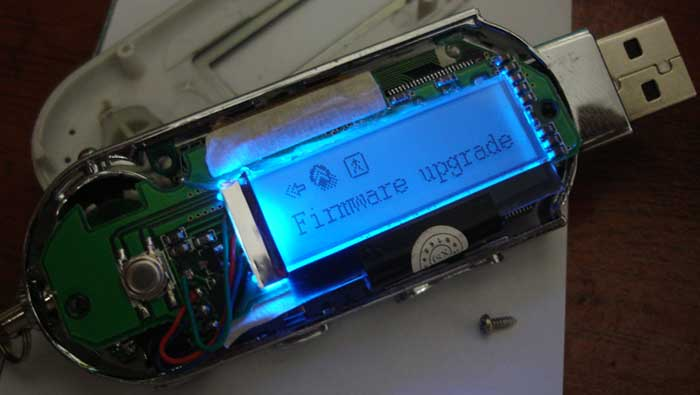
\includegraphics[height=2cm]{res/Firmware_upgrade.jpg} \cite{firmwareUpgrade}
\end{frame}

\begin{frame}{PID 1}
	Nachdem Linux alles initializiert hat wird Kontrolle an Userspace uebergeben.
	Ueblicherweise ist dies systemd.
	\begin{itemize}
		\item systemd
		\begin{itemize}
			\item einfach da bekannt
			\item wenn mehrere Dienste noetig
			\item gewisse groesse
		\end{itemize}
		\item script
		\begin{itemize}
			\item wenn nur wenige Dienste
		\end{itemize}
		\item applikation
		\begin{itemize}
			\item Applikation muss alles machen
			\item nur fuer monolithische Applikationen
		\end{itemize}
	\end{itemize}
\end{frame}

\begin{frame}{Yocto}
	Aufgaben um Embedded system zu erstellen
	\begin{itemize}
		\item Cross Compiler bauen
		\item sysfs bauen (Kernel und benoetigte Tools fuer system)
		\item Cross Compiler und sysfs fuer Developer bereitstellen (sdk)
	\end{itemize}
	Aufgaben um Embedded system zu deployen
	\begin{itemize}
		\item Applikation cross-compilen
		\item sysfs cross-compilen
		\item Kernel cross-compilen
		\item applikationen packetieren
		\item image zusammenstellen
	\end{itemize}
	daher Yocto (Yocto Workflow zeigen, resp. bild aus fsfe präsentation)
\end{frame}

\begin{frame}{Kernel / Linux}
	\begin{itemize}
		\item Verteilen von Resourcen
		\item Initialisieren und Abstrahieren der Hardware
	\end{itemize}
\end{frame}

\begin{frame}{Device Tree}
	\begin{itemize}
		\item meiste Hardware ist nicht Plug and Play
		\item wir muessen Linux mitteilen, wo welche Hardware liegt
		\item Device Tree listet auf, wo sich welche Hardware befindet
		\item Linux laedt Treiber anhand Infos in Device Tree
	\end{itemize}
	\begin{itemize}
		\item Struktur aehnlich wie XML
		\item gegliedert nach BUS
		\item beschreibt welche Hardwrae angeschlossen ist
		\item Hierarchisch aufgebaut wie Hardware (SOC, Modul, Geraet, System)
	\end{itemize}
	Beispiel
\end{frame}


\begin{frame}{Sonstiges}
	\begin{itemize}
		\item[busybox] Reimplementation von GNU/Linux Tools in einem Binary, optimiert auf groesse; oft eingeschraenker Funktionsumfang
	\end{itemize}
\end{frame}

\begin{frame}{important to know}
opkg -o /opt/mume/1.8.1/sysroots/cortexa8hf-vfp-neon-poky-linux-gnueabi/ install ~/projekte/yocto/mume/build/tmp/deploy/ipk/cortexa8hf-vfp-neon/libtinyxml*
\end{frame}

\section{Literatur \& Bild-Nachweise}
\begin{frame}[allowframebreaks]{Literature}
	\tiny{
		\bibliography{literature}
	}
\end{frame}

}

\end{document}
